\documentclass[../differential_methods.tex]{subfiles}
\begin{document}
\section{Aula 07 - 23 de Março, 2026}
\subsection{Motivações}
\begin{itemize}
	\item Método Vermelho-azul;
	\item Gauss-Seidel e Jacobi;
	\item Métodos Iterativos sem Matrizes.
\end{itemize}
\subsection{Organização de Sistemas}
Veremos um método de organização de sistemas de variáveis desconhecidas chamado \textbf{numeração vermelho-azul}\footnote{Na verdade, é vermelho-preto, mas  parte em preto fica pintada em azul porque todo o resto do texto já é preto; então, eu decidi colocar vermelho-azul para não sofrer o efeito Stroop.}; nele, a ideia é escrever as equações em uma cor, contendo variáveis em vermelho, e depois escrever as outras equações em cor azul, sendo as variáveis vermelhas conectadas às azuis apenas pelo estêncil laplaciano de 5-pontos.
\begin{figure}[H]
	\begin{center}
		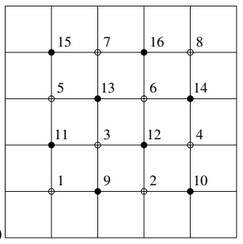
\includegraphics[height=0.35\textheight, width=0.35\textwidth, keepaspectratio]{./Images/red_black_07.png}
	\end{center}
	\caption{variáveis vermelhas-azuis ordenadas em uma malha 4x4 com condições de Dirichlet; os pontos não pintados são vermelhos, e os pintados são azuis.}
\end{figure}

O sistema resultante pode ser escrito, então, como
\[
	\begin{bmatrix}
		D     & H \\
		H^{T} & D
	\end{bmatrix} \begin{bmatrix}
		{\color{Red2} U_{r}} \\
		{\color{Blue2} U_{b}}
	\end{bmatrix} = \begin{bmatrix}
		{\color{Red2}f_{r}} \\
		{\color{Blue2}f_{b}}
	\end{bmatrix},
\]
onde
\[
	D = \frac{1}{h^{2}}\begin{bmatrix}
		-4 &    &        &    \\
		   & -4 &        &    \\
		   &    & \ddots &    \\
		   &    &        & -4
	\end{bmatrix}
\]
e H é uma matriz com zeros e uns, multiplicados por \(\frac{1}{h^{2}}\), cuja estrutura depende na geometria da malha.

Essa técnica tira vantagem do fato de que computar \(D^{-1}\) ser computacionalmente bem barato; note que, pelo sistema resultante, obtemos as equações
\begin{align*}
	 & D{\color{Red2}U_{r}}+H{\color{Blue2}U_{b}}={\color{Red2}f_{r}}       \\
	 & H^{T}{\color{Red2}U_{r}}+D{\color{Blue2}U_{b}}={\color{Blue2}f_{b}},
\end{align*}
de forma que, ao isolarmos o termo \({\color{Red2}U_{r}}\), obtemos a relação
\[
	{\color{Red2}U_{r}}=-D^{-1}H{\color{Blue2}U_{b}}+D^{-1}{\color{Red2}f_{r}}.
\]
Com a relação acima, podemos substituir os termos nas equações obtidas da matriz, obtendo:
\[
	H^{T}(-D^{-1}H{\color{Blue2}U_{b}}+D^{-1}{\color{Red2}f_{r}})+D{\color{Blue2}U_{b}}={\color{Blue2}f_{b}} \Rightarrow (D-H^{T}D^{-1}H){\color{Blue2}U_{b}}={\color{Blue2}f_{b}}-H^{T}D^{-1}{\color{Red2}f_{r}},
\]
o qual pode ser reescrito como \(B{\color{Blue2}U_{b}}=g\), tendo metade das equações do sistema original, mas sendo fácil de construir B e g. Assim, basta resolver esse sistema e as variáveis vermelhas poderão ser obtidas muito mais facilmente, sem resolver sistemas lineares! Logo, caso ele possa ser implementado, o peso computacional economiza o tempo computacional para resolver o sistema pela metade!!

O próximo passo é aplicar esse método à equação elíptica. Pela expansão de Taylor, segue que
\begin{align*}
	\nabla_{5}^{2}u(x_{i}, y_{j}) & =\nabla^{2}u(x_{i}, y_{j})+\frac{1}{12}h^{2}\frac{\partial^{4}u}{\partial x^{4}}(x_{i}, y_{j})+\frac{1}{12}h^{2}\frac{\partial^{4}u}{\partial y^{4}}(x_{i}, y_{j})+\mathcal{O}(h^{4})                                                                                                                                \\
	                              & \Rightarrow \nabla_{5}^{2}u(x_{i}, y_{j})+{\color{SpringGreen4}\frac{2}{12}h^{2}\frac{\partial^{4}u}{\partial y^{2}\partial x^{2}}(x_{i}, y_{j})}                                                                                                                                                                    \\
	                              & = \nabla^{2}u(x_{i}, y_{j})+\frac{1}{12}h^{2}\underbrace{\biggl[\frac{\partial^{4}u}{\partial x^{4}}(x_{i}, y_{j}) + {\color{SpringGreen4}2\frac{\partial^{4}u}{\partial x^{2}\partial y^{2}}(x_{i}, y_{j})} + \frac{\partial^{4}u}{\partial y^{2}}(x_{i}, y_{j})\biggr]}_{{\color{Red2} \nabla^{4}u(x_{i}, y_{j})}} \\
	                              & = \nabla^{2}u(x_{i}, y_{j})+{\color{Red2}\frac{1}{12}h^{2}\nabla^{2}\nabla^{2}f(x_{i}, y_{j})}+\mathcal{O}(h^{4})                                                                                                                                                                                                    \\
	                              & \Rightarrow \nabla_{5}^{2}u(x_{i}, y_{j})+{\color{SpringGreen4}\frac{2}{12}h^{2}\frac{\partial^{4}u}{\partial y^{2}\partial x^{2}}(x_{i}, y_{j})}-{\color{Red2}\frac{1}{12}h^{2}\nabla^{2}f(x_{i}, y_{j})}                                                                                                           \\
	                              & =\nabla^{2}u(x_{i}, y_{j})+\mathcal{O}(h^{4}).
\end{align*}
Podemos proceder ainda mais nesse raciocínio e obter uma aproximação com 9 pontos:
\begin{align*}
	            & \nabla_{5}^{2}u(x_{i}, y_{j})+{\color{SpringGreen4}\frac{2}{12}h^{2}\frac{\partial^{4}u}{\partial y^{2}\partial x^{2}}(x_{i}, y_{j})}-{\color{Red2}\frac{1}{12}h^{2}\nabla^{2}f(x_{i}, y_{j})} =\nabla^{2}u(x_{i}, y_{j})+\mathcal{O}(h^{4})  \\
	\Rightarrow & \nabla_{5}^{2}u(x_{i}, y_{j})+{\color{SpringGreen4}\frac{h^{2}}{6h^{4}}\biggl[u(x_{i-1}, y_{j-1})-2u(x_{i-1}, y_{j}) + u(x_{i-1}, y_{j+1})-2u(x_{i}, y_{j-1})                                                                               } \\
	            & {\color{SpringGreen4}+4u(x_{i}, y_{j})-2u(x_{i},y_{j+1})+u(x_{i+1}, y_{j-1})-2u(x_{i+1}, y_{j})+u(x_{i+1},y_{j+1})\biggr]+\mathcal{O}(h^{4})}                                                                                                 \\
	            & {\color{Red2}-\frac{1}{12}h^{2}\nabla^{2}f(x_{i}, y_{j})}=\nabla^{2}u(x_{i}, y_{j})+\mathcal{O}(h^{4}).
\end{align*}
Portanto, a aproximação
\begin{align*}
	\nabla_{9}^{2}U_{ij} & \coloneqq \frac{1}{6h^{2}}[4U_{i-1, j}+4U_{i+1, j}+4U_{i, j-1}+4U_{i, j+1}+U_{i-1, j} + U_{i-1, j+1}+U_{i+1, j-1} \\
	                     & +4U_{i+1, j+1}-20U_{ij}] = f_{ij}+\frac{1}{12}h^{2}\nabla^{2}f(x_{i}, y_{j})
\end{align*}
constitui um esquema de diferenças finitas para o problema de Poisson com erro de truncamento local \(\mathcal{O}(h^{4})\), e o termo \(\displaystyle \frac{1}{12}h^{2}\nabla^{2}f(x_{i}, y_{j}) \) pode ser computado de forma exata, ou aproximado por \(\displaystyle \frac{1}{12}h^{2}\nabla_{5}^{2}f(x_{i}, y_{j})\).
\begin{figure}[H]
	\begin{center}
		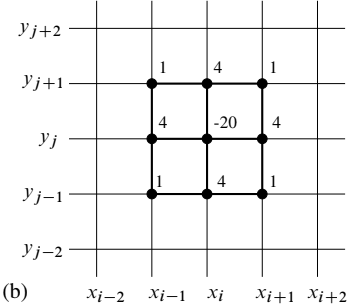
\includegraphics[height=0.35\textheight, width=0.35\textwidth, keepaspectratio]{./Images/nine_stencil_07.png}
	\end{center}
	\caption{estêncil de 9 pontos para o Laplaciano em torno do ponto \((x_{i}, y_{j})\) com pesos indicados.}
\end{figure}
\subsection{Estimativas por Diferentes Fontes}
Suponha que temos o desejo de obter uma solução verdadeira, denote por \(E(h)\) a função erro em uma malha de tamanho h, por \(U(h)\) o vetor da solução numérica, e \(\hat{U}(h)\) a solução verdadeira avaliada na mesma grade, tais que
\[
	E(h)=\Vert U(h)-\hat{U}(h) \Vert.
\]

Se o método tem precisão de ordem p, ou seja, se conforme \(h\to 0\),
\[
	E(h)=Ch^{p}+\mathcal{O}(h^{p+1}),
\]
então para \(0<h_2<h_1\) suficientemente pequenos, espera-se que
\[
	E(h_{1})\approx Ch_{1}^{p} \quad\&\quad E(h_{2})\approx Ch_{2}^{p}.
\]
Assim, a ordem de convergência pode ser estimada, tal qual fora feito no início do curso, pela expressão
\[
	p\approx \frac{\log^{}{\biggl(\frac{E(h_1)}{E(h_2)}\biggr)}}{\log^{}{\biggl(\frac{h_1}{h_2}\biggr)},}
\]
pois
\[
	\log^{}{\biggl(\frac{E(h_1)}{E(h_2)}\biggr)}\approx \log^{}{\biggl(\frac{Ch_{1}^{p}}{Ch_{2}^{p}}\biggr)}=\log^{}{\biggl(\frac{h_1}{h_2}\biggr)^{p}}=p\log^{}{\biggl(\frac{h_1}{h_2}\biggr)}.
\]

Esse tipo de estimativa é conhecida como \textbf{estimativa a partir da solução verdadeira}, mas não a u única fonte: podemos obter, também, uma \textbf{estimativa pela solução com malha fina}, por exemplo, na quL não sabemos a solução exata, mas podemos rodar o problema por uma malha fina, digamos \(\overline{h}\), e usar a solução numérica obtida \(U(\overline{h})\) como referência.
Neste contexto, seja \(U(h)\) a solução numérica em uma malha mais grossa, com tamanho h, e \(\overline{U}(h)\) ser a restrição de \(U(\overline{h})\) à h-malha; observe como
\[
	U(h)-\overline{U}(h)=(U(h)-\hat{U}(h))+(\hat{U}(h)-\overline{U}(h))
\]
leva à estimativa
\[
	\Vert U(h)-\overline{U}(h) \Vert \leq \underbrace{\Vert U(h)-\hat{U}(h) \Vert}_{E(h)} + \underbrace{\Vert \hat{U}(h)-\overline{U}(h) \Vert}_{\overline{E}(h)}.
\]
Além disso, como \((\overline{h})^{p}<<h^{p}\), necessariamente deve ocorrer
\[
	\overline{E}(h)=\Vert \hat{U}(h)-\overline{U}(h) \Vert \approx \Vert U(\overline{h})-\hat{U}(\overline{h}) \Vert = E(\overline{h})<<E(h),
\]
ou seja, podemos assumir sem grandes receios que \(\Vert U(h)-\overline{U}(h) \Vert\) é uma boa aproximação do erro verdadeiro \(E(h)\)!

Para as funções de grades, temos as seguintes normas \(L^{p}\):
\begin{itemize}
	\item \textbf{Norma \(\mathbf{L^{p}}\):} dado que \(U(x)\) é uma aproximação da solução \(u(x)\) no fechado \(\overline{\Omega }=[a, b]\), denotemos por \(e(x)\coloneqq U(x)-u(x)\), onde \(U(x)\) e \(u(x)\) são suficientemente suaves, a diferença da aproximação para a solução real. Então, definimos:
	      \[
		      \Vert e \Vert_{L^{\infty}(\Omega )}\coloneqq \max\limits_{a\leq x\leq b}| e(x) | \quad\&\quad \Vert e \Vert_{L^{p}(\Omega )} = \biggl(\int_{a}^{b}| e(x) |^{p} \mathrm{d}x\biggr)^{\frac{1}{p}},\; p\geq 1;
	      \]
	\item \textbf{Norma \(\mathbf{L^{p}}\) Discreta para Função Grade Unidimensional:} sejam \(U_{i}\approx u(x_{i})\) e \(e_{i}=U_{i}-u(x_{i})\), onde \(1\leq i\leq n\). Definimos
	      \[
		      \Vert e \Vert_{\infty}\coloneqq \max\limits_{1\leq i\leq N}| e_{i} | \quad\&\quad \Vert e \Vert_{p}\coloneqq \biggl(h \sum\limits_{i=1}^{N}| e_{i} |^{p} \mathrm{d}x\biggr)^{\frac{1}{p}}, \; p\geq 1;
	      \]
	\item \textbf{Norma \(\mathbf{L^{p}}\) Discreta para Função Grade Bidimensional:} sejam \(U_{ij}\approx u(x_{i}, y_{j})\) e \(e_{ij}=U_{ij}-u(x_{i}, y_{j})\), com \(1\leq i\leq M\) e \(1\leq j\leq N\); então, definimos
	      \[
		      \Vert e \Vert_{\infty}\coloneqq \max\limits_{\substack{1\leq i\leq M \\ 1\leq j\leq N}| e_{ij} |}\quad\&\quad \Vert e \Vert_{p}\coloneqq \biggl(\Delta x\Delta y \sum\limits_{i=1}^{M}\sum\limits_{j=1}^{N}| e_{ij} |^{p}\mathrm{d}x\biggr)^{\frac{1}{p}},\; p\geq 1.
	      \]
\end{itemize}

Estamos suficientemente equipados para lidar com métodos iterativos sem matrizes! A ideia, aqui, é isolar  \(U_{i,j}\) em termos de outras variáveis:
\[
	U_{i, j}=\frac{1}{4}(U_{i-1, j}+U_{i+1, j} + U_{i, j-1}+U_{i, j+1})-\frac{h^{2}}{4}f_{i, j},
\]
permitindo criarmos um novo processo iterativo para produzir uma nova estimativa, denotada por \(U_{i, j}^{[k+1]},\) baseada em valores já conhecidos \(U_{i, j}^{[k]}\), que pode ser resumido na expressão
\[
	U_{i, j}^{[k+1]}=\frac{1}{4}(U_{i-1, j}^{[k]}+U_{i+1, j}^{[k]}+U_{i, j-1}^{[k]}+U_{i, j+1}^{[k]})-\frac{h^{2}}{4}f_{i, j},
\]
conhecido como \textbf{Iteração de Jacobi para o Problema de Poisson}.
O primeiro detalhe observável é que não há a necessidade de armazenar uma matriz esparsa, mas sim dar um palpite inicial \(U_{i, j}^{[0]}\); por isso, esse método iterativo converge \textbf{muito devagar} para uma solução discreta do problema de Poisson, independente do chute inicial dado! Além disso, ela pode ser modificada para incorporar condições de fronteira de Neumann ou de Robin sem dar vontade de chorar em posição fetal por horas.
\begin{figure}[H]
	\begin{center}
		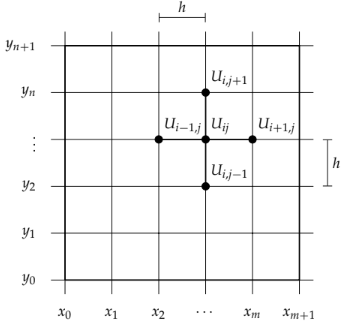
\includegraphics[height=0.35\textheight, width=0.35\textwidth, keepaspectratio]{./Images/jacobi_07.png}
	\end{center}
\end{figure}

Outro método sem matrizes que vale a pena mencionar é o \textbf{Método Iterativo de Gauss-Seidel para Problemas de Poisson}; nele, utiliza-se os valores computados disponíveis mais recentemente obtidos durante a iteração na malha, resultando em
\[
	U_{i, j}^{[k+1]} = \frac{1}{4}(U_{i-1, j}^{[k+1]} + U_{i+1, j}^{[k]}+U_{i, j-1}^{[k+1]}+U_{i, j+1}^{[k]})-\frac{h^{2}}{4}f_{i, j},
\]
sendo que as mesmas considerações do método anterior permanecem ativas aqui.
\begin{figure}[H]
	\begin{center}
		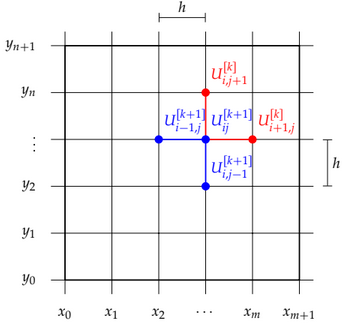
\includegraphics[height=\textheight, width=\textwidth, keepaspectratio]{./Images/gauss_seidel_07.png}
	\end{center}
	\caption{}
\end{figure}

Tanto o método de Gauss-Seidel, quanto o de Jacobi, são facilmente implementáveis, com custo de armazenamento ótimos; porém, eles são conhecidos justamente por sua lentidão para convergir durante o processo iterativo, no sentido de levar muitas e muitas iterações, às vezes mais de milhares, para conseguir uma aproximação razoável, além de ser mais difícil de vetorizar as computações (talvez o Matlab leve vantagem sobre o Python por conta disso para esses métodos).

\end{document}
